\subsubsection{アーキテクチャ測度}
\keyterm{アーキテクチャ測度}\en{architecture metrics}とは、アーキテクチャの性質を数量で表すものである。測度は万能ではないが、複雑さ、依存関係、変更リスク、規約適合性を把握する手がかりになる。

代表的な測度には、構成要素間依存、循環依存、循環的複雑度、内部モジュール複雑度、結合度、凝集度、ネストの深さ、パターン・様式・API への準拠などがある。

継続的開発や DevOps の文脈では、アーキテクチャそのものではなく、アーキテクチャの状態を反映する過程測度も使われる。変更リードタイム、配置頻度、サービス復旧平均時間、変更失敗率などである。変更が遅く、復旧が難しく、失敗率が高い場合、アーキテクチャが変更や運用に適していない可能性がある。

\begin{figure}[htbp]
\centering
\IfFileExists{swebok_structure/CH02.ソフトウェアアーキテクチャ(Software_Architecture)/2.4.ソフトウェアアーキテクチャ評価(Software_Architecture_Evaluation)/2.4.4.アーキテクチャ測度(Architecture_Metrics)/assets/fig-ch02-09.png}{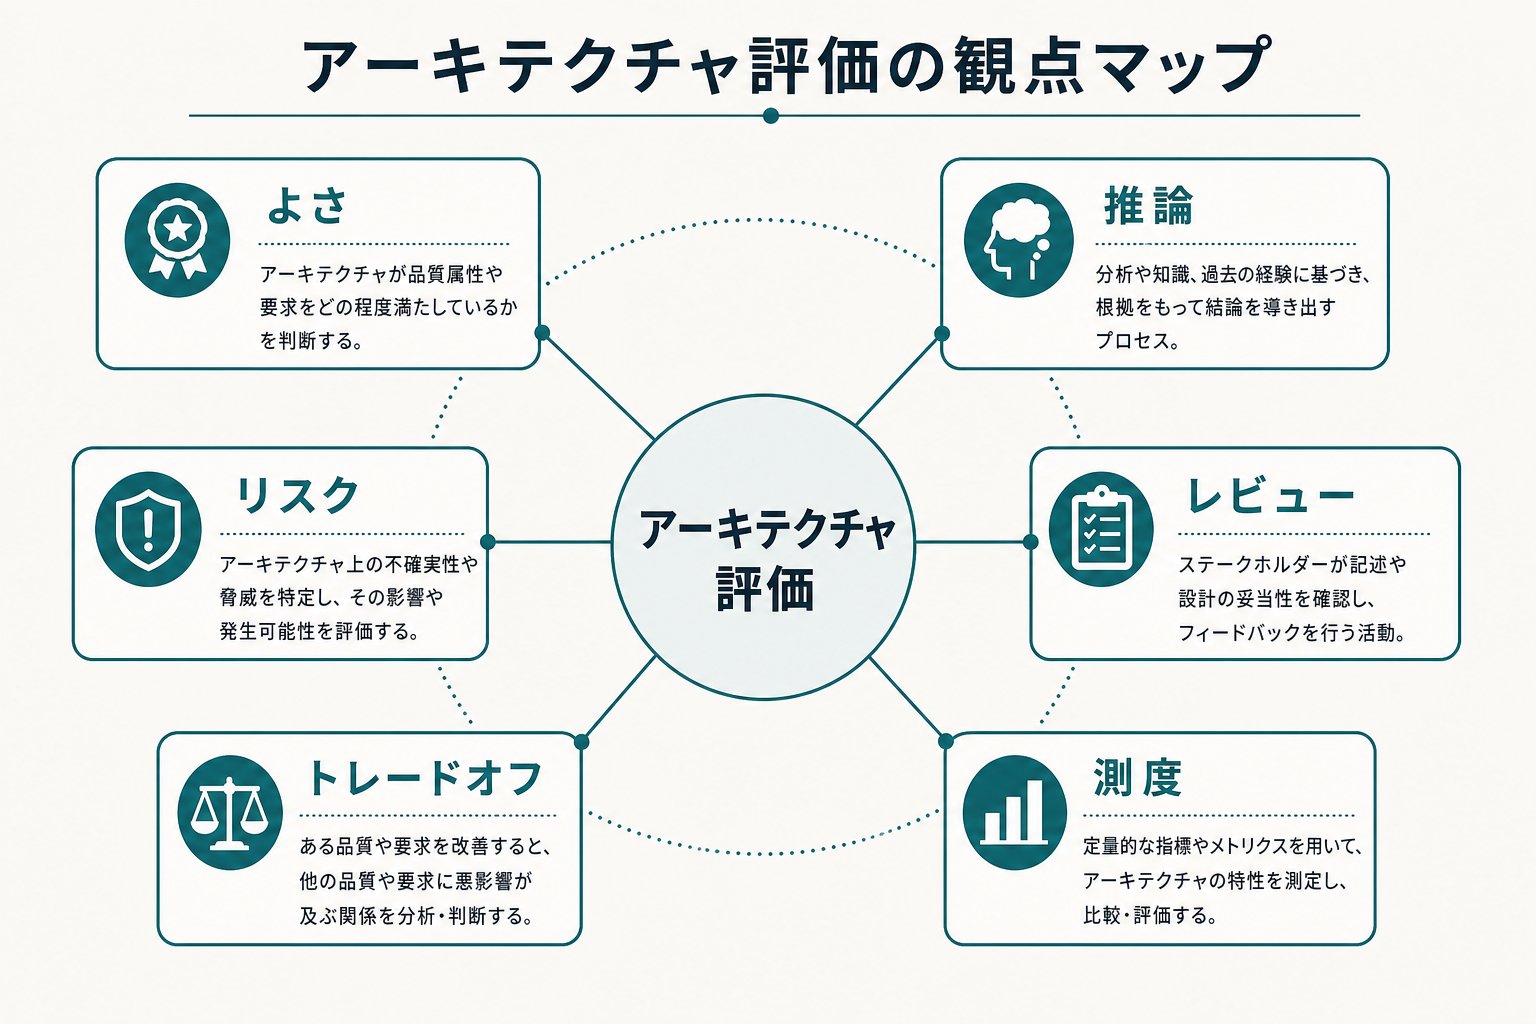
\includegraphics[width=0.96\linewidth]{swebok_structure/CH02.ソフトウェアアーキテクチャ(Software_Architecture)/2.4.ソフトウェアアーキテクチャ評価(Software_Architecture_Evaluation)/2.4.4.アーキテクチャ測度(Architecture_Metrics)/assets/fig-ch02-09.png}}{\fbox{\parbox[c][48mm][c]{0.9\linewidth}{\centering 画像生成待ち\\アーキテクチャ評価の観点マップ}}}
\caption{アーキテクチャ評価の観点マップ}
\label{fig:ch02-09}
\end{figure}
